\documentclass[12pt]{article}
\usepackage[english]{babel}
\usepackage{array}
\usepackage{setspace}
\usepackage{graphicx}
\usepackage{sistyle} %\num{100000} for commas
\SIthousandsep{,}
\usepackage{fancyhdr}
\usepackage{listings} % For code listings, may break stuff
\usepackage{xcolor, diagbox, empheq, makecell, tcolorbox}
\usepackage[autostyle]{csquotes}
\usepackage{amssymb, amsthm, linguex, enumitem, amsmath}
\usepackage{tcolorbox} %dont know what this does
\usepackage[colorlinks=true, allcolors=blue]{hyperref}
\usepackage{lipsum}

\makeatletter   %% <- make @ usable in macro names
\newcommand*\notab[1]{%
  \begingroup   %% <- limit scope of the following changes
    \par        %% <- start a new paragraph
    \@totalleftmargin=0pt \linewidth=\columnwidth
    %% ^^ let other commands know that the margins have been reset
    \parshape 0
    %% ^^ reset the margins
    #1\par      %% <- insert #1 and end this paragraph
  \endgroup
}
\makeatother    %% <- revert @

\pagestyle{empty}

\textwidth 6.5in
\hoffset=-.65in
\textheight=9.5in
\voffset=-1.in

%Sets
\newcommand{\R}{\mathbb{R}}
\newcommand{\C}{\mathbb{C}}
\newcommand{\N}{\mathbb{N}}
\newcommand{\F}{\mathbb{F}}
\newcommand{\Z}{\mathbb{Z}}
\newcommand{\Cb}{\mathbf{C}}
\newcommand{\Fb}{\mathbf{F}}
\newcommand{\Rb}{\mathbf{R}}

%Misc

\newcommand{\pars}[1]{\left( {#1} \right) } %auto size parenthesis 
\newcommand{\brac}[1]{\left[ {#1} \right] } %auto size brackets around arg
\newcommand{\set}[1]{\left\{{#1}\right\}} %auto size curly braces around arg
\newcommand{\vbrac}[1]{\left\langle{#1}\right\rangle} %vector angle brackets
\newcommand{\inner}[1]{\left\langle{#1}\right\rangle} %vector angle brackets
\newcommand{\conj}[1]{\overline{{#1}}} %conjugate bar
\newcommand{\vconj}[1]{\overline{\vbrac{{#1}}}}
\newcommand{\ceil}[1]{\left\lceil {#1} \right\rceil} %auto size ceiling around arg
\newcommand{\floor}[1]{\left\lfloor {#1} \right\rfloor} %auto size floor around arg

\newcommand{\limn}{\lim_{n\to\infty}} %limit as n approaches infinity
\newcommand{\thru}[1]{{#1}_1, \dots, {#1}_n}
\newcommand{\sumthru}[1]{{#1}_1 + \cdots + {#1}_n}
\renewcommand{\over}[1]{\frac{1}{{#1}}}
\newcommand{\pfrac}[2]{\left( \frac{{#1}}{{#2}} \right) } %auto size parenthesis over fraction 
\newcommand{\pover}[1]{\left( \frac{1}{{#1}} \right) } %auto size parenthesis over fraction

%Boolean Algebra
\newcommand{\OR}{\,\lor\,}
\newcommand{\AND}{\,\land\,}

%Probability and Statistics
\newcommand{\xbar}{\bar{X}}
\newcommand{\ybar}{\bar{Y}}
\newcommand{\yn}{Y_1, \dots, Y_n}
\newcommand{\yx}{X_1, \dots, X_n}
\newcommand{\normDist}{N\left(\mu, \sigma^2\right)} %default normal distribution
\newcommand{\gammaDist}[2]{\operatorname{Gamma} \left( {#1},{#2} \right)}
\newcommand{\norm}[1]{\left\| {#1} \right\|}
\newcommand{\abs}[1]{\left| {#1} \right|}
\newcommand{\prob}[1]{P \left( {#1} \right) }
\newcommand{\E}[1]{E \left( {#1} \right) }
\newcommand{\Eb}[1]{E[ \,{#1}\, ]} %E bracket
\newcommand*{\V}[1]{V \left( {#1} \right) }
\newcommand{\Vb}[1]{V [ \,{#1}\, ] }
\newcommand{\that}{\hat{\theta}} %theta hat
\newcommand{\phat}{\hat{p}}
\newcommand{\psihat}{\hat{\psi}}
\newcommand{\Psihat}{\hat{\Psi}}


\newcommand{\dimrange}[1]{\operatorname{dim}\operatorname{range}{#1}} % dimrange
\newcommand{\dimnull}[1]{\operatorname{dim}\operatorname{null}{#1}} % dimnull

\newcommand{\vdub}[2]{\begin{pmatrix}{#1}\\{#2}\end{pmatrix}}

%Linear Algebra
\newcommand{\poly}[1]{\mathcal{P}_{#1}(\mathbf{R})} %polynomial up to degree (arg)
\newcommand{\pf}{\mathcal{P}(\mathbf{F})} %set of all polynomials
\renewcommand{\L}[1]{\mathcal{L}\left({#1}\right)}%Set of linear maps
\newcommand{\vdouble}[2]{\begin{pmatrix}{#1}\\{#2}\end{pmatrix}} % 2 high vertical
\newcommand{\vtriple}[3]{\begin{pmatrix}{#1}\\{#2}\\{#3}\end{pmatrix}} %vertical vector parenthesis, 3 args
\newcommand{\vquad}[4]{\begin{pmatrix}{#1}\\{#2}\\{#3}\\{#4}\end{pmatrix}} %vertical vector parenthesis, 4 args
\newcommand{\vquin}[5]{\begin{pmatrix}{#1}\\{#2}\\{#3}\\{#4}\\{#5}\end{pmatrix}} %vertical vector parenthesis, 5 args
\newcommand{\vvector}[3]{\begin{bmatrix}{#1}\\{#2}\\{#3}\end{bmatrix}} %vertical vector braces, 3 args
\newcommand{\dimn}[1]{\operatorname{dim}\,{#1}}
\newcommand{\rank}[1]{\operatorname{dim}\operatorname{range}{#1}}
\newcommand{\nullity}[1]{\operatorname{dim}\operatorname{null}{#1}}
\newcommand{\range}[1]{\operatorname{range}{#1}}
\newcommand{\NULL}[1]{\operatorname{null}{#1}}
\renewcommand{\null}{\operatorname{null}}
\newcommand{\mat}[4]{\begin{bmatrix}{#1} & {#2}\\{#3}&{#4}\end{bmatrix}} % 2x2 matrix
\newcommand{\Mat}[9]{\begin{bmatrix}{#1} & {#2} & {#3}\\{#4}&{#5}&{#6}\\{#7}&{#8}&{#9}\end{bmatrix}} % 3x3 matrix
\newcommand{\detx}[4]{\begin{vmatrix}{#1} & {#2}\\{#3}&{#4}\end{vmatrix}} % 2x2 determinant
\newcommand{\nf}{\infty}
%colors
\definecolor{ggreen}{RGB}{0, 127, 0}
\definecolor{dgray}{RGB}{63,63,63}
\definecolor{neonorange}{RGB}{255,47,0}
\definecolor{mygray}{rgb}{0.5,0.5,0.5}
\newcommand{\red}[1]{\color{red}{#1}\color{black}}
\newcommand{\grn}[1]{\color{ggreen}{#1}\color{black}}
\newcommand{\blu}[1]{\color{blue}{#1}\color{black}}
\newcommand{\redx}[1]{\color{red}\not{#1}\color{black}}

\newcommand{\say}[1]{\textquotedblleft{#1}\textquotedblright} %quote the "argument"
\newcommand*\widefbox[1]{\fbox{\hspace{2em}#1\hspace{2em}}}
\newtcolorbox{mybox}[1][]{colback=white, sharp corners, #1}

%Line break spacings
\newcommand{\nl}{\vspace{0.1in}\noindent}
\newcommand{\nnl}{\vspace{0.2in}\noindent}
\newcommand{\nnnl}{\vspace{0.3in}\noindent}

% Code snippets
\newcommand*{\code}{\fontfamily{qcr}\selectfont}
\lstset{
    backgroundcolor=\color{white},
    basicstyle=\footnotesize,
    breakatwhitespace=false,         % sets if automatic breaks should only happen at whitespace
    breaklines=true,                 % sets automatic line breaking
    captionpos=b,                    % sets the caption-position to bottom
    commentstyle=\color{dgray},    % comment style
    deletekeywords={...},            % if you want to delete keywords from the given language
    escapeinside={(*@}{@*)},          % if you want to add LaTeX within your code
    extendedchars=true,              % lets you use non-ASCII characters; for 8-bits encodings only, does not work with UTF-8
    firstnumber=1,                % start line enumeration with line 1
    frame=single,	                   % adds a frame around the code
    keepspaces=true,                 % keeps spaces in text, useful for keeping indentation of code (possibly needs columns=flexible)
    keywordstyle=\color{neonorange},       % keyword style
    language=C++,                 % the language of the code
    morekeywords={*,...},            % if you want to add more keywords to the set
    numbers=left,                    % where to put the line-numbers; possible values are (none, left, right)
    numbersep=5pt,                   % how far the line-numbers are from the code
    numberstyle=\tiny\color{mygray}, % the style that is used for the line-numbers
    rulecolor=\color{black},         % if not set, the frame-color may be changed on line-breaks within not-black text (e.g. comments (green here))
    showspaces=false,                % show spaces everywhere adding particular underscores; it overrides 'showstringspaces'
    showstringspaces=false,          % underline spaces within strings only
    showtabs=false,                  % show tabs within strings adding particular underscores
    stringstyle=\color{purple},     % string literal style
    tabsize=4,	                   % sets default tabsize to 4 spaces
}

\lstdefinestyle{cpp}{language=C++,
    morekeywords={cout, cin, Comparable, T},numbers=none
}
%Examples:
%{\code while}
%
%{\code \begin{lstlisting}[language=C++]
%sum1 = 0;
%for (i = 1; i <= n; i *= 2)
%    for (j = 1; j <= n; j++)
%        sum1++;
%\end{lstlisting}}







\begin{document}

\pagestyle{fancy}
\fancyhf{}
\fancyhead[RO]{Matthew Wilder} %header top right
\fancyhead[LO]{MTH 326 - Homework \#6} %header top left
\fancyfoot[CO]{Page \thepage} %page center bottom

\noindent MTH 326 - Spring 2022
\\Assignment \#6
\\Due: Wednesday March 9, 2022 (11:59pm)

\begin{enumerate}
    \item Suppose that we want to study whether students enrolled in a campus wellness program get more sleep than the average college student.  (This problem assumes that the wellness group comes from the same general population as the other college students.)  Suppose that the average student gets 6.1 hours of sleep per day and denote $\mu$ denote the average sleep gotten by a student in the wellness population.
\begin{enumerate}[label=(\alph*)]
    \item State the hypothesis test for the test you are designing.
    \begin{mybox}
        \textbf{Solution: }

        \nl We are testing whether the wellness group gets \textit{more} sleep than the general population. Hence, we are testing $\mu_a > \mu_0$. The null hypothesis is that there is no difference in means, thus $\mu_a = \mu_0$. 
        \begin{align*}
            H_0 &: \mu_0 = \mu_a
            \\ H_a &: \mu_0 < \mu_a
        \end{align*}
    \end{mybox}
\end{enumerate}
Assume the standard \textit{deviation} is known as $\sigma=0.5$ hour and that the underlying sleep distribution is normal and that there are 16 students in the wellness program.  We define the rejection region to be $\bar{Y}>6.3$.
\begin{enumerate}[label=(\alph*)]
    \setcounter{enumii}{1}
    \item Find $\alpha$, the probability of Type I error.
    \begin{mybox}
        \textbf{Solution: }

        \nl We will show the probability that $H_0$ is rejected when it is true. (df = 15)
        \begin{align*}
            \alpha &= \Pr(\text{Type I error})\\
            &= \Pr(\ybar > 6.3 \mid \mu_0 = 6.1)\\
            &= \Pr\pars{t > \frac{6.3-6.1}{0.5 \big/ \sqrt{16}}}\\
            &= \Pr(t > 1.6)\\
            &\approx 0.065223 \tag{By WA \say{technology}}
        \end{align*}
        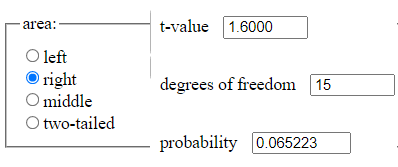
\includegraphics[height=1.5in]{p1b.PNG}
    \end{mybox}
\newpage
    \item Find $\beta$, the probability of Type II error at $\mu=6.3, 6.5,$ and $6.7$.
    \begin{mybox}
        \textbf{Solution: }

        \nl For the probability of a Type 2 error, we want the left tail probability.

        \nl When $\mu = 6.3,$
        $$\mathcal{T}= \frac{\ybar - \mu}{S \big/\sqrt{n}} = \frac{6.3-6.3}{0.5 \big/\sqrt{15}} = 0$$
        And $\Pr(\mathcal{T} < 0) = 0.5$.\\ $\beta = 0.5$ \\\_\_\_\_\_\_\_\_\_\_\_\_\_\_\_\_\_\_\_\_\_\_\_\_\_\_\_\_\_\_\_\_\_\_\_\_\_\_\_\_\_\_\_\_\_\_\_\_\_\_\_\_\_\_\_\_\_\_\_\_\_\_\_\_\_\_\_\_\_\_\_\_\_\_\_\_\_\_\_\_\_\_\_\_\_\_\_\_\_\_\_
        
        
        \nnl When $\mu = 6.5,$
        $$\mathcal{T}= \frac{\ybar - \mu}{S \big/\sqrt{n}} = \frac{6.3-6.5}{0.5 \big/\sqrt{15}} = -1.54919$$
        And $\Pr(Z < -1.54919) \approx 0.071087$.

        \noindent 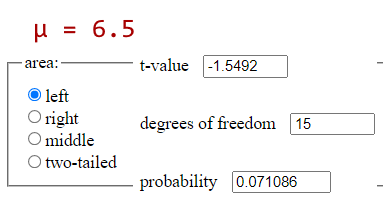
\includegraphics[height=1.5in]{165.PNG}
        \\ $\beta = 0.071087$\\
        \_\_\_\_\_\_\_\_\_\_\_\_\_\_\_\_\_\_\_\_\_\_\_\_\_\_\_\_\_\_\_\_\_\_\_\_\_\_\_\_\_\_\_\_\_\_\_\_\_\_\_\_\_\_\_\_\_\_\_\_\_\_\_\_\_\_\_\_\_\_\_\_\_\_\_\_\_\_\_\_\_\_\_\_\_\_\_\_\_\_\_
        
        \nnl When $\mu = 6.7,$
        $$\mathcal{T}= \frac{\ybar - \mu}{S \big/\sqrt{n}} = \frac{6.3-6.7}{0.5 \big/\sqrt{15}} = -3.09838$$
        And $\Pr(Z < -3.09838) \approx 0.003671$.

        \noindent 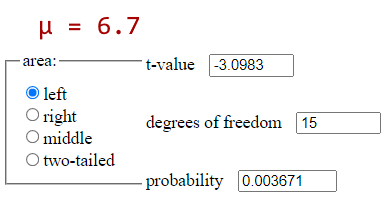
\includegraphics[height=1.5in]{166.PNG}
        \\ $\beta = 0.003671$
    \end{mybox}
    \newpage
    \item Sketch the power function for this test.
    
    \nnl \textbf{Solution: } The following Desmos graph is has the \red{red } line as the power function $\red{\operatorname{power}(\theta) = 1-\beta(\theta)}$. This is approximately the same shape as the respective T distribution with 15 degrees of freedom, but was easier to set up the integral with normal.
    \makeatletter
    \begingroup   %% <- limit scope of the following changes
    \par        %% <- start a new paragraph
    \@totalleftmargin=0pt \linewidth=\columnwidth
    %% ^^ let other commands know that the margins have been reset
    \parshape 0
    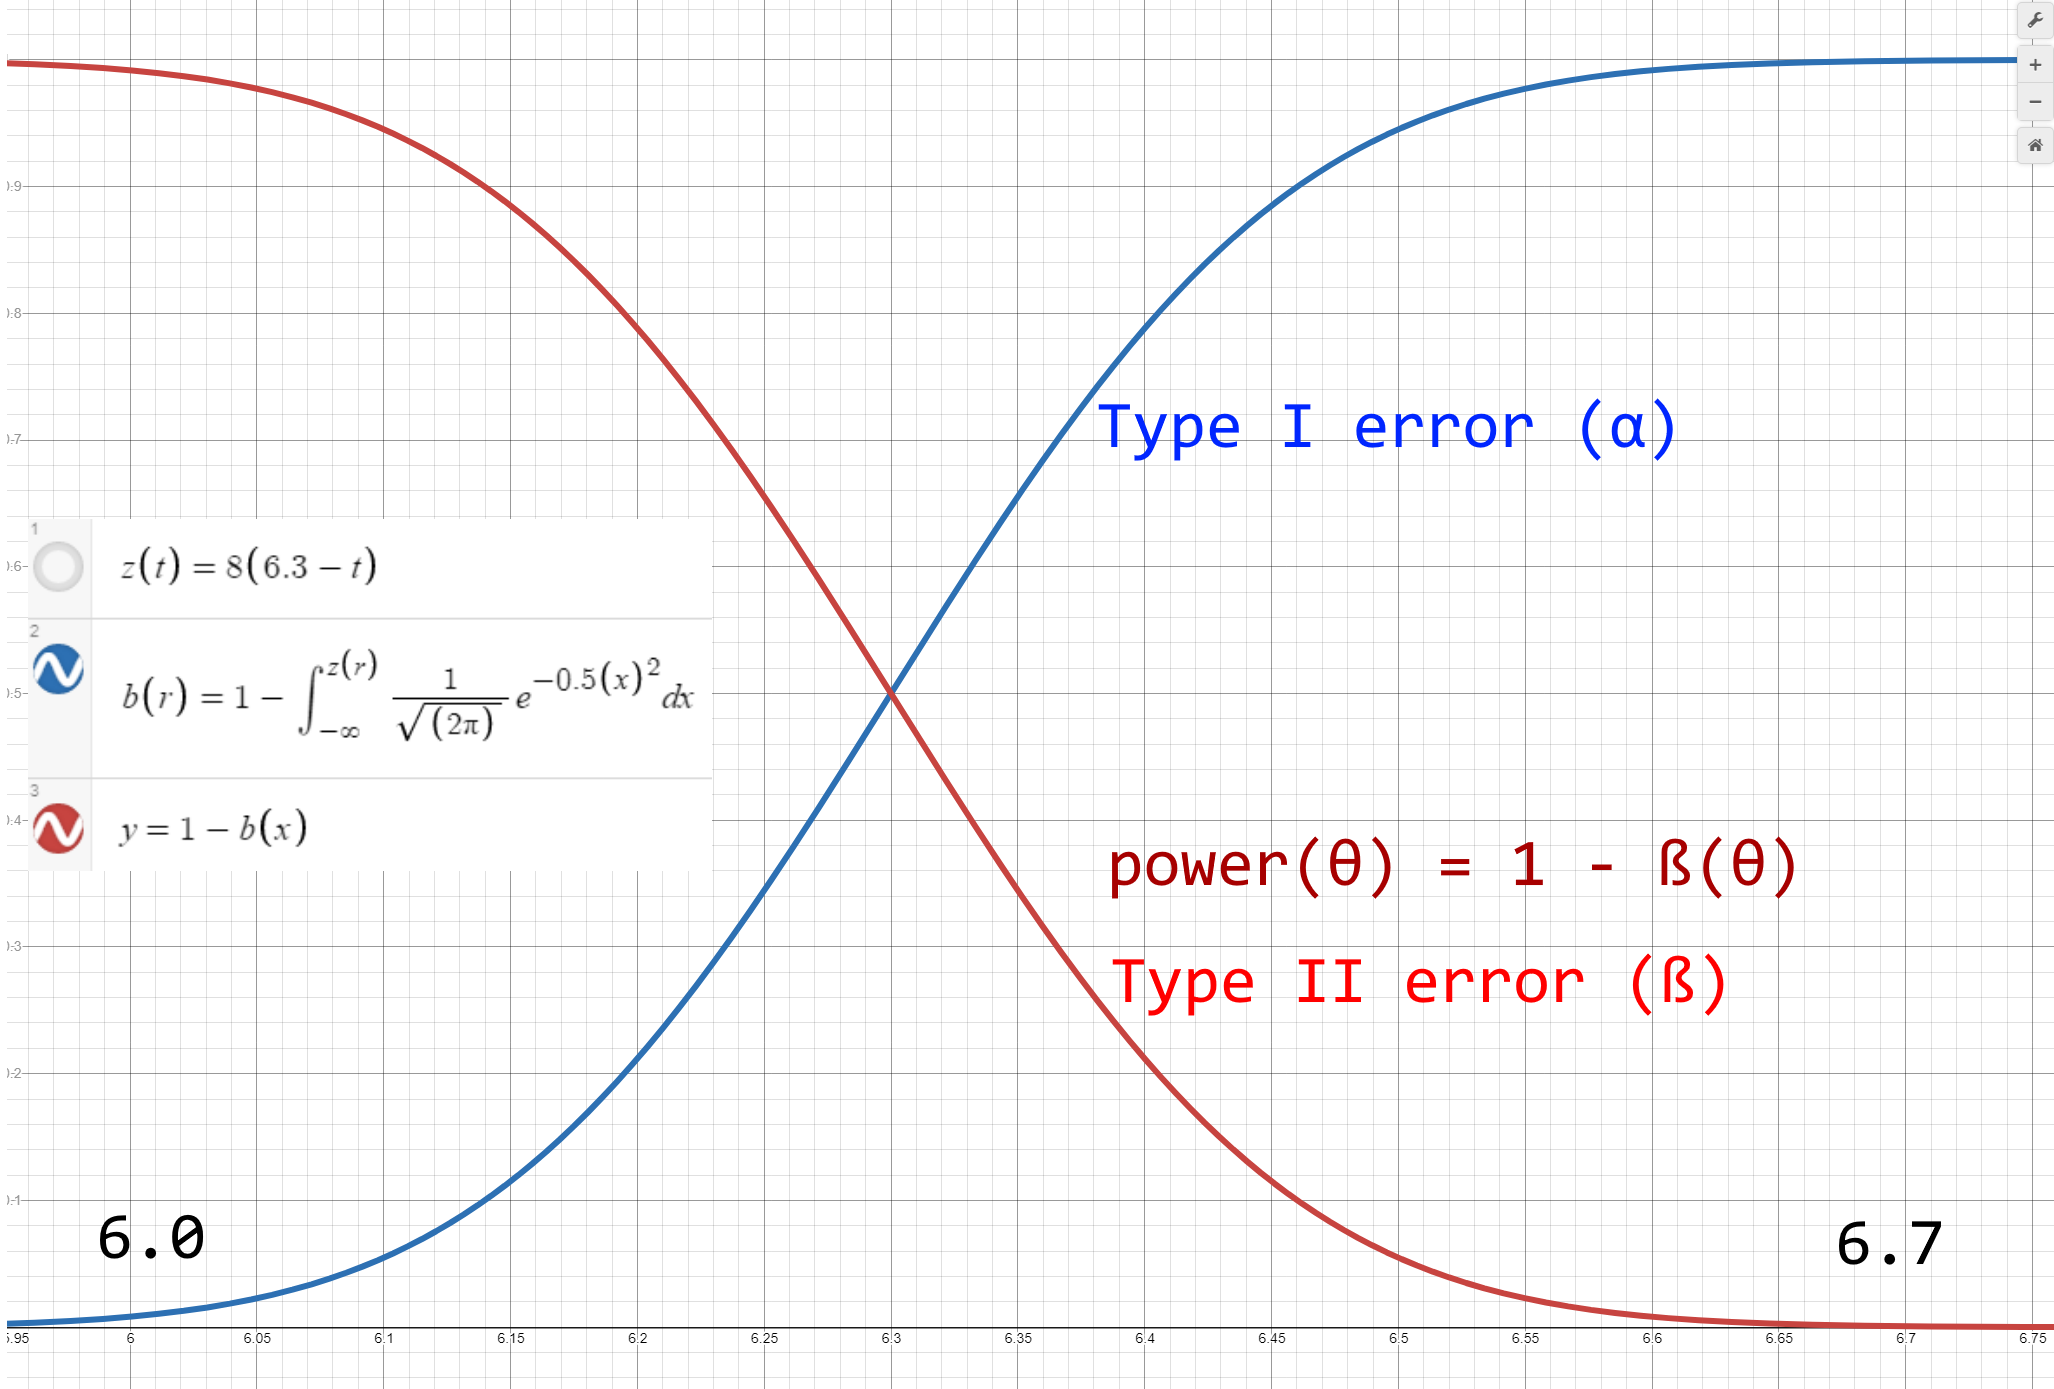
\includegraphics[width=6.5in]{prob1.PNG}
    %% ^^ reset the margins
    \par      %% <- insert #1 and end this paragraph
  \endgroup
    
\end{enumerate}
    \newpage
    \item Lifetimes of certain brand of switch follows (approximately) a normal distribution with mean 100 hours.  Five switches of a new brand are obtained and tested and their lifetimes measured to be 120, 101, 114, 95, and 130 hours.  Does this provide strong evidence that the new switches have a longer average lifespan?
\begin{mybox}
    \textbf{Solution:} 
    \begin{align*}
        H_0 &: \mu_0 = 100 \text{ hours}
        \\ H_a &: \mu_a > 100 \text{ hours} 
    \end{align*}
    
    The sample mean is $\mu = 112$. The sample standard deviation is
    \begin{align*}
        S^2 &= \dfrac{\sum(x_i-\bar{x})^2}{n-1}\\
        &= \frac{(95-112)^2 + (101-112)^2 + (114-112)^2 + (120-112)^2 + (130-112)^2}{5-1}  \\ &= 200.5
    \end{align*}
    and $S \approx 14.1598$. Then our test statistic is
    $$\mathcal{T} = \frac{\xbar - \mu}{S \big/ \sqrt{n}} = \frac{112-100}{14.1598 \big/ \sqrt{5}} \approx 1.895.$$
    Using an $\alpha = 0.01$ significance level with $n-1 = 4$ degrees of freedom. Via Table 5, $t_{0.005}(4) = 4.604$. The respective $p$ value is
    \begin{align*}
        p &= \Pr(\mathcal{T} \geq 1.895 \mid \mu_0 = 100)\\
        &< \Pr(\mathcal{T} \geq 4.604)\\
        &= 0.005  \tag{WebAssign \say{technology}}\\
        &< \alpha
    \end{align*}
    Hence, we reject $H_0$ and conclude that there is sufficient evidence that the\\ lifespan has increased.
    \noindent \begin{center}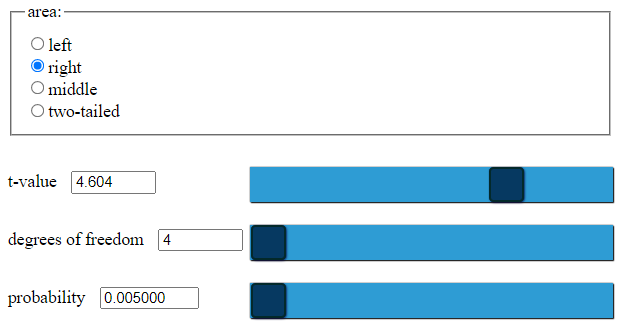
\includegraphics[width=4.5in]{p2.PNG}
    \end{center}
\end{mybox}
    \newpage
    \item A federal regulatory agency hypothesises that the average length of a stay in the hospital is in excess of 5 days.  A pilot data set had standard \textit{deviation} of 3.1 days.  Using this as the population standard error, how large a sample would you need in designing a test with $\alpha=0.01$ and $\beta=0.05$ if the true average is 5.5 days.

\begin{mybox}
    \textbf{Solution:} We assume this follows a normal distribution and let 
    \begin{align*}
        H_0 &: \mu_0 = 5
        \\ H_a &: \mu_a = 5.5
    \end{align*}
    Then $Z_{\alpha} = Z_{0.01} \approx 2.33$ and $Z_{\beta} = Z_{0.05} \approx 1.645$.
    Using the following formula,
    $$n = \ceil{ \pfrac{Z_{\alpha}+Z_{\beta}}{\mu_a - \mu_0}^2 \cdot S^2 }$$
    we can substitute in our data to obtain
    $$n = \ceil{\pfrac{2.33 + 1.645}{5.5-5}^2 \cdot 3.1^2 } = \ceil{607.376} = 608.$$
    Therefore the sample will need to be at least size $n = 608$.
\end{mybox}

    \vspace{.35in}
    \item A study was performed to compare two cholesterol-reducing drugs.  Observations of the number of units of cholesterol reduction were recorded for 12 subjects receiving Drug A and 14 subjects receiving Drug B:
\begin{center}
\begin{tabular}{|l|c|c|}
  \hline
  % after \\: \hline or \cline{col1-col2} \cline{col3-col4} ...
  \  & \textbf{Drug A} & \textbf{Drug B} \\\hline
  $n$ & 12  & 14 \\
  Mean & 5.64 & 5.03 \\
  stnd \textit{deviation} & 1.25 & 1.82 \\
  \hline
\end{tabular}
\end{center}
Researchers are interested in testing if the drugs appear to be \emph{different} in their average cholesterol reduction.
\begin{enumerate}
    \item State the assumptions needed for the independent samples $t$ test to be valid.
    \begin{mybox}
        \textbf{Solution:}
        \begin{itemize}
            \item Population must be at least 20 times the sample size
            \item The variance of the two populations are the same.
            \item The two random samples are independent.
            \item The samples were selected from normal populations.
        \end{itemize}
        
    \end{mybox}
    \newpage
    \item Perform the $t$-test, find the $p$-value, and state the conclusion using a 5\% significance level.
    \begin{mybox}
        \textbf{Solution:} Using the pooled estimator, and since we assume $\mu_0 = \mu_a$ then $\mu_0 - \mu_a = 0$.
        $$S_p^2 = \dfrac{\displaystyle \sum(X_i - \xbar)^2 + \sum(Y_i-\ybar)^2}{n_1 + n_2 -2}.$$
        $$T = \dfrac{(\xbar-\ybar)-(\mu_X-\mu_Y)}{S_p \displaystyle \sqrt{\dfrac{1}{n_1} + \dfrac{1}{n_2}}}.$$

            $$\displaystyle \frac{\left(5.64-5.03\right)-0}{\sqrt{\dfrac{\left(12-1\right)\cdot 1.25^2+\left(14-1\right)\cdot 1.82^2}{12+14-2}}\sqrt{\dfrac{1}{12}+\dfrac{1}{14}}} \approx 0.97865.$$
            
            \nl Using technology, $p = 0.337516$ Since $p > \alpha = 0.05$ we accept $H_0$ and conclude that there is \textbf{not} enough evidence to indicate a difference between the two drugs.

            \noindent \begin{center}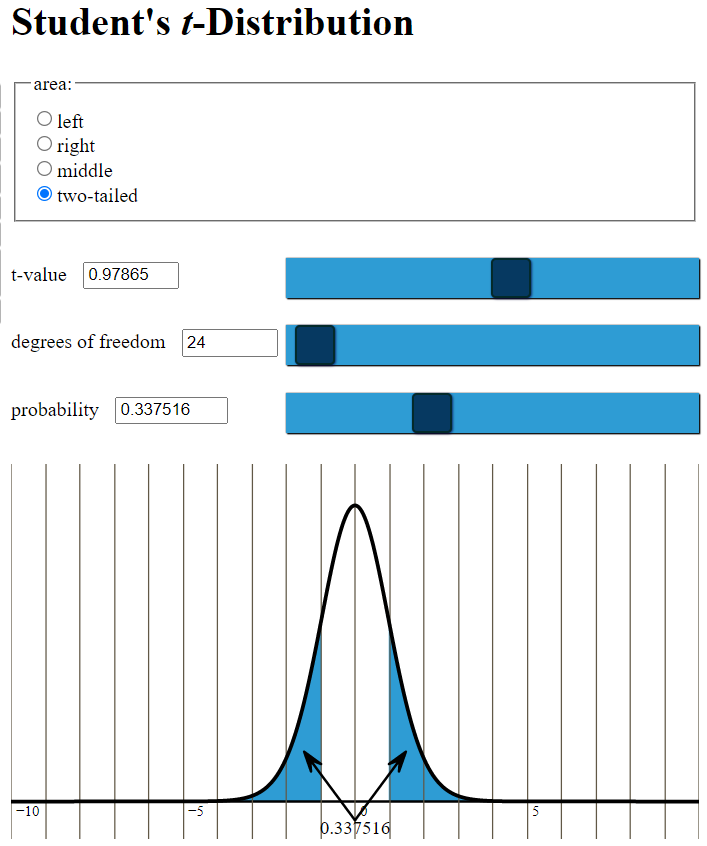
\includegraphics[width=4.5in]{p42.PNG}
            \end{center}

            
    \end{mybox}
\end{enumerate}
    \end{enumerate}
\end{document} 